\tikzset{every picture/.style={line width=0.75pt}} %set default line width to 0.75pt        

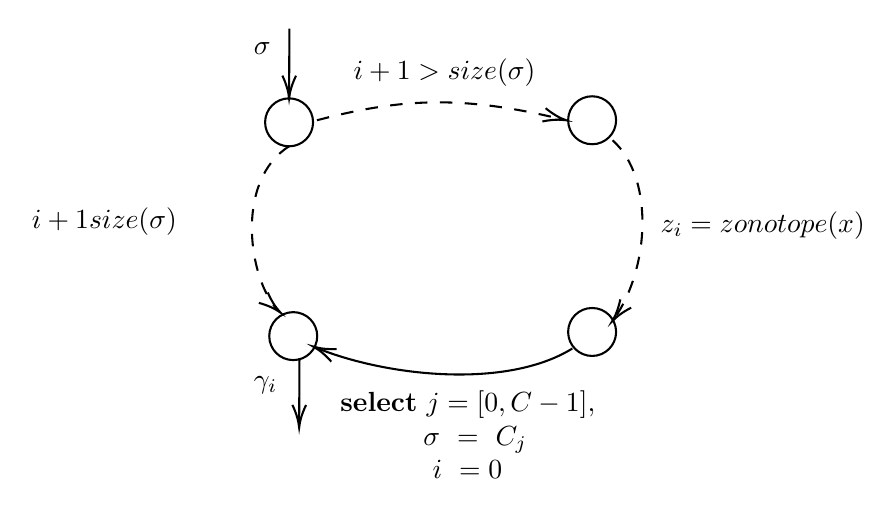
\begin{tikzpicture}[x=0.75pt,y=0.75pt,yscale=-1,xscale=1]
%uncomment if require: \path (0,464); %set diagram left start at 0, and has height of 464

%Shape: Circle [id:dp8712375528286049] 
\draw   (232.89,150.55) .. controls (232.89,144.17) and (238.06,139) .. (244.45,139) .. controls (250.83,139) and (256,144.17) .. (256,150.55) .. controls (256,156.94) and (250.83,162.11) .. (244.45,162.11) .. controls (238.06,162.11) and (232.89,156.94) .. (232.89,150.55) -- cycle ;
%Shape: Circle [id:dp0053736784066187315] 
\draw   (378.89,251.55) .. controls (378.89,245.17) and (384.06,240) .. (390.45,240) .. controls (396.83,240) and (402,245.17) .. (402,251.55) .. controls (402,257.94) and (396.83,263.11) .. (390.45,263.11) .. controls (384.06,263.11) and (378.89,257.94) .. (378.89,251.55) -- cycle ;
%Shape: Circle [id:dp7786102631576663] 
\draw   (378.89,149.55) .. controls (378.89,143.17) and (384.06,138) .. (390.45,138) .. controls (396.83,138) and (402,143.17) .. (402,149.55) .. controls (402,155.94) and (396.83,161.11) .. (390.45,161.11) .. controls (384.06,161.11) and (378.89,155.94) .. (378.89,149.55) -- cycle ;
%Curve Lines [id:da06892458990894723] 
\draw  [dash pattern={on 4.5pt off 4.5pt}]  (257.89,149.55) .. controls (299.47,138.66) and (328.31,137.57) .. (376.43,149.2) ;
\draw [shift={(377.89,149.55)}, rotate = 193.76] [color={rgb, 255:red, 0; green, 0; blue, 0 }  ][line width=0.75]    (10.93,-3.29) .. controls (6.95,-1.4) and (3.31,-0.3) .. (0,0) .. controls (3.31,0.3) and (6.95,1.4) .. (10.93,3.29)   ;
%Curve Lines [id:da34373825883144815] 
\draw  [dash pattern={on 4.5pt off 4.5pt}]  (244.45,162.11) .. controls (218.1,178.69) and (224.84,226.23) .. (238.96,240.93) ;
\draw [shift={(240.29,242.2)}, rotate = 220.91] [color={rgb, 255:red, 0; green, 0; blue, 0 }  ][line width=0.75]    (10.93,-3.29) .. controls (6.95,-1.4) and (3.31,-0.3) .. (0,0) .. controls (3.31,0.3) and (6.95,1.4) .. (10.93,3.29)   ;
%Curve Lines [id:da0893746859182114] 
\draw  [dash pattern={on 4.5pt off 4.5pt}]  (400.29,159.2) .. controls (420.72,177.37) and (417.97,221.4) .. (401.05,245.13) ;
\draw [shift={(400,246.55)}, rotate = 307.39] [color={rgb, 255:red, 0; green, 0; blue, 0 }  ][line width=0.75]    (10.93,-3.29) .. controls (6.95,-1.4) and (3.31,-0.3) .. (0,0) .. controls (3.31,0.3) and (6.95,1.4) .. (10.93,3.29)   ;
%Shape: Circle [id:dp610189050328179] 
\draw   (234.89,253.55) .. controls (234.89,247.17) and (240.06,242) .. (246.45,242) .. controls (252.83,242) and (258,247.17) .. (258,253.55) .. controls (258,259.94) and (252.83,265.11) .. (246.45,265.11) .. controls (240.06,265.11) and (234.89,259.94) .. (234.89,253.55) -- cycle ;
%Curve Lines [id:da6066202102744167] 
\draw    (380.89,259.55) .. controls (348.78,279.35) and (291.05,272.86) .. (257.52,259.18) ;
\draw [shift={(256,258.55)}, rotate = 382.95] [color={rgb, 255:red, 0; green, 0; blue, 0 }  ][line width=0.75]    (10.93,-3.29) .. controls (6.95,-1.4) and (3.31,-0.3) .. (0,0) .. controls (3.31,0.3) and (6.95,1.4) .. (10.93,3.29)   ;
%Straight Lines [id:da9519097834156862] 
\draw    (249.45,264.11) -- (249.3,295.65) ;
\draw [shift={(249.29,297.65)}, rotate = 270.27] [color={rgb, 255:red, 0; green, 0; blue, 0 }  ][line width=0.75]    (10.93,-3.29) .. controls (6.95,-1.4) and (3.31,-0.3) .. (0,0) .. controls (3.31,0.3) and (6.95,1.4) .. (10.93,3.29)   ;
%Straight Lines [id:da75432083913083] 
\draw    (244.6,105.45) -- (244.46,137) ;
\draw [shift={(244.45,139)}, rotate = 270.27] [color={rgb, 255:red, 0; green, 0; blue, 0 }  ][line width=0.75]    (10.93,-3.29) .. controls (6.95,-1.4) and (3.31,-0.3) .. (0,0) .. controls (3.31,0.3) and (6.95,1.4) .. (10.93,3.29)   ;

% Text Node
\draw (422,192.04) node [anchor=north west][inner sep=0.75pt]    {$z_{i} =zonotope( x)$};
% Text Node
\draw (274,118.4) node [anchor=north west][inner sep=0.75pt]    {$i+1 >size( \sigma )$};
% Text Node
\draw (119,190.4) node [anchor=north west][inner sep=0.75pt]    {$i+1\leqslant size( \sigma )$};
% Text Node
\draw (226,110.4) node [anchor=north west][inner sep=0.75pt]    {$\sigma $};
% Text Node
\draw (226,271.4) node [anchor=north west][inner sep=0.75pt]    {$\gamma _{i}$};
% Text Node
\draw (261,277.4) node [anchor=north west][inner sep=0.75pt]    {$ \begin{array}{l}
\mathbf{select} \ j=[ 0,C-1] ,\\
\ \ \ \ \ \ \ \ \ \sigma \ =\ C_{j}\\
\ \ \ \ \ \ \ \ \ \ i\ =0\\
\end{array}$};


\end{tikzpicture}
